\documentclass[UTF8,a4paper]{ctexart}
\usepackage[utf8]{inputenc}
\usepackage{amsmath}
\usepackage{pdfpages}
\usepackage{graphicx}
\usepackage{wrapfig}
\usepackage{listings}
\usepackage{xcolor}
\lstset{
    numbers=left, 
    numberstyle= \tiny, 
    keywordstyle= \color{ blue!70},
    commentstyle= \color{red!50!green!50!blue!50}, 
    frame=shadowbox, % 阴影效果
    rulesepcolor= \color{ red!20!green!20!blue!20} ,
    escapeinside=``, % 英文分号中可写入中文
    xleftmargin=2em,xrightmargin=2em, aboveskip=1em,
    framexleftmargin=2em
} 
\title{模式识别作业5 BP算法的实现}
\author{张蔚桐\ 2015011493\ 自55}
\begin {document}
\maketitle
首先推导$\delta$函数
根据题中设置的损失函数可以知道,稀疏项S对第二层网络没有影响,因此第一层网络采用题目中给出的$\delta$函数,第二层网络的$\delta$可以迅速求出,相对经典的$\delta$配置多出$\lambda W$

对表达式进行向量——矩阵化可以得到性能较好的算法,采用默认的参数配置对神经网络进行训练可以得到比较好的训练结果

训练采样的图片集为图\ref{ori}所示,而生成的图片集为图\ref{out}所示

程序训练时间为19s
\begin{figure}
\centering
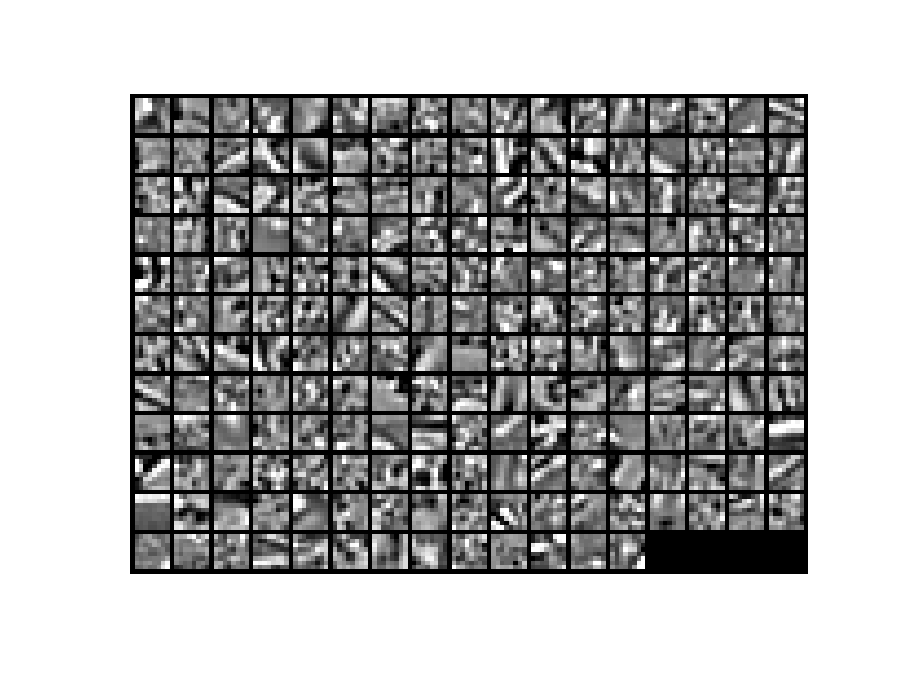
\includegraphics[width=\textwidth]{starter/ori.eps}
\caption{随机产生的训练集}
\label{ori}
\includegraphics[width=\textwidth]{starter/weights.jpg}
\caption{训练成果集}
\label{out}
\end{figure}
\end{document}